\documentclass{article}
\usepackage{CJKutf8, indentfirst, graphicx, subfigure}
\begin{document}
\begin{CJK}{UTF8}{bsmi}
\title{硬體設計與實驗 Lab4 Report}
\author{
104021219 鄭余玄
}
\date{}
\maketitle
\section{實做過程}
clock\_divider 在 lab3 實做的時候,
我是使用參數化的寫法,
因此能快速的產出 clk/$2^{13}$ 和 clk/$2^{25}$ 這兩個訊號。

debounce 電路是參考老師投影片的寫法,
不過我使用更精簡的 behaviorial 的描述,
使用 \{ 和 \} 就可以接合訊號了。

lab2\_2 修改的地方只有 clock trigger 的方式,
把原本的 negedge 改成 posedge 而已。
至於 en 的開始和暫停,我是寫在 lab4 程式碼中。
在 lab4 的程式碼加上一個 enable 訊號,
當每次有 debounced en 訊號時,
就反轉一次,就可以達到開始和暫停的效果。

在 lab4\_1 中,因為只會顯示最後一個位數,
所以 Seven Segment Decoder 比較特別一點,
DIGIT 就只需要輸出 1110,
因此整個七段顯示器電路是一個 combinational circuit。
lab4\_1 最後就只需要將那些電路接一接,
就可以完成了。

在 lab4\_2 中,
Seven Segment Decoder 會需要快速切換,
利用視覺暫留感覺好像同時顯示兩個位數。
此外,用兩個 BCD 顯示兩位數的方法,
是將第一個 cout 訊號,
接到第二個的 en 訊號,
因此當每次要進位時,
第二個 BCD 就會數一次。

lab4\_3 的 min 和 max 訊號,
是使用 BCD 判斷是否是顯示 99 或是 0。
而至於 BCD 計數方向是否要反向,
我是利用 BCD 判斷是否是 98 或是 1。
這應該是很關鍵的點,
因為如果是判斷 99 或是 0 的話,
會晚一個 clock,這樣輸出就不對了。

\subsection{Block diagram}
\begin{figure*}[]
\centering{
\hfill
  \subfigure[]{ \label{fig:sub1}
  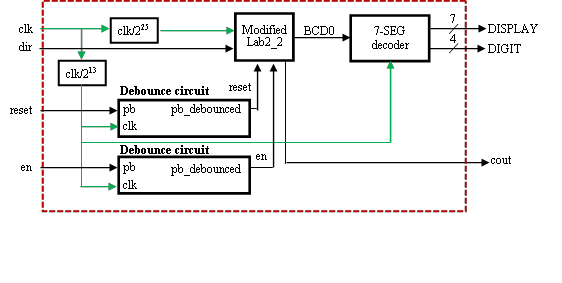
\includegraphics[width=.7\textwidth, angle=0]{lab4_1}
}
\hfill
  \subfigure[]{ \label{fig:sub2}
    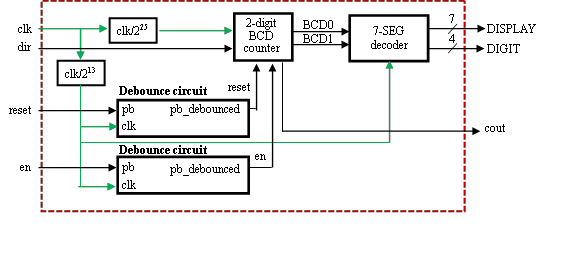
\includegraphics[width=.7\textwidth, angle=0]{lab4_2}
  }
\hfill
  \subfigure[]{ \label{fig:sub3}
    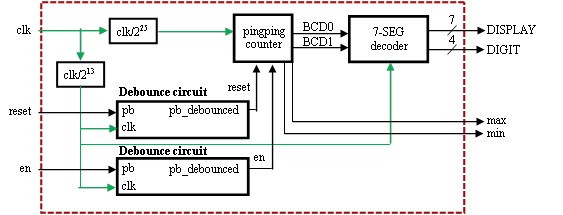
\includegraphics[width=.7\textwidth, angle=0]{lab4_3}
  }
}
\caption{Block diagrams: (a) lab4\_1 (b) lab4\_2 and (c) lab4\_3.}
\end{figure*}
基本上照著圖想,程式幾乎不會有什麼錯。

\section{學到的東西及遇到的困難}
這次是第一次知道 debounce 電路怎麼寫,
不過是出乎我意料之外的簡單,
原來只需要取幾個樣本點,
就判定現在的電壓是否是穩定的。
不過我有稍微問過老師,
老師是說有沒有 debounce,
其實感覺不是很明顯,
效果不是很顯著。

因為之前電機系室友有修邏輯設計,
所以我稍微知道有 debounce 和七段顯示器的原理。
這次學到最多大概就是,
把那些電路寫成 verilog 程式碼吧。
這次實驗也沒有遇到太大的困難。

\section{想對老師或助教說的話}
我覺得老師可以參考我的 debounce 電路的寫法,
雖然作法一樣,不過是有稍微更簡潔了一些。

老師投影片中的 DISPLAY 訊號 MSB,
和 Basys3\_Master.xdc 的順序不同,
因此當初在接的時候,
那些數字就好像變成亂碼了。

Basys3\_Master.xdc 提供的四個七段顯示器埠口中,
有一個 V7 埠,我原本還在想說那要接什麼,
後來才發現原來那是中間的冒號不用接。

\end{CJK}
\end{document}
